\subsection{Introduction} \label{p2introduction}

%\begin{itemize}
%  \item Evolutionary approaches to design of dungeons
%  \item Different criteria evaluated in dungeons
%  \begin{itemize}
%  	\item Criteria evaluated for evolutionary approaches
%  \end{itemize}
%  \item What we present in the paper  Techniques and changes. How is the paper divided
%\end{itemize}

%Procedural content generation (PCG) has been widely used to generate content in games for different reasons, due to constraints in memory~\citepsecond{p2Braben1984Elite}, create new experiences for the user~\citepsecond{p2Toy1980Rogue}, animations~\citepsecond{p2Maxis2008Spore} or more recently, to create most of the assets~\citepsecond{p2HelloGames2016NoSky}. Moreover, the interest on PCG has increased since researchers explore ways to automatize, reduce cost and, produce novel and interesting content, for instance, weapons~\citepsecond{p2Hastings2009GalacticGame}, levels~\citepsecond{p2Shaker2012EvolvingEvolution}, music and sound~\citepsecond{p2Hoover2011InteractivelyScaffolding,Scirea2017PImprovisation}, generators \citepsecond{p2Liapis2013SentientAuthoring} and even complete commercial games with their own rules \citepsecond{p2Browne2007Yavalath}.
Procedural content generation (PCG) has been widely used to generate content in games for different reasons, due to constraints in memory~\citepsecond{p2Braben1984Elite}, create new experiences for the user~\citepsecond{p2Toy1980Rogue}, animations~\citepsecond{p2Maxis2008Spore} or more recently, to create most of the assets~\citepsecond{p2HelloGames2016NoSky}. Moreover, interest in PCG has increased as researchers have explored ways to automate, reduce cost and, produce novel and interesting content, for instance, weapons~\citepsecond{p2Hastings2009GalacticGame}, levels~\citepsecond{p2Shaker2012EvolvingEvolution}, music and sound~\citepsecond{p2Hoover2011InteractivelyScaffolding,p2Scirea2017PImprovisation}, and even complete commercial games~\citepsecond{p2Browne2007Yavalath}.

Search-based procedural content generation (SBPCG) is a popular PCG approach that uses evolutionary algorithms (EA) for guiding the content generation process by means of evaluation functions~\citepsecond{p2Shaker2016TheApproach}. Mixed-initiative SBPCG involves human users in the evolutionary process so that promotes the co-creation of human and machine-made designs \citepsecond{p2Liapis2013SentientAuthoring}.

% \begin{figure}[H]
% 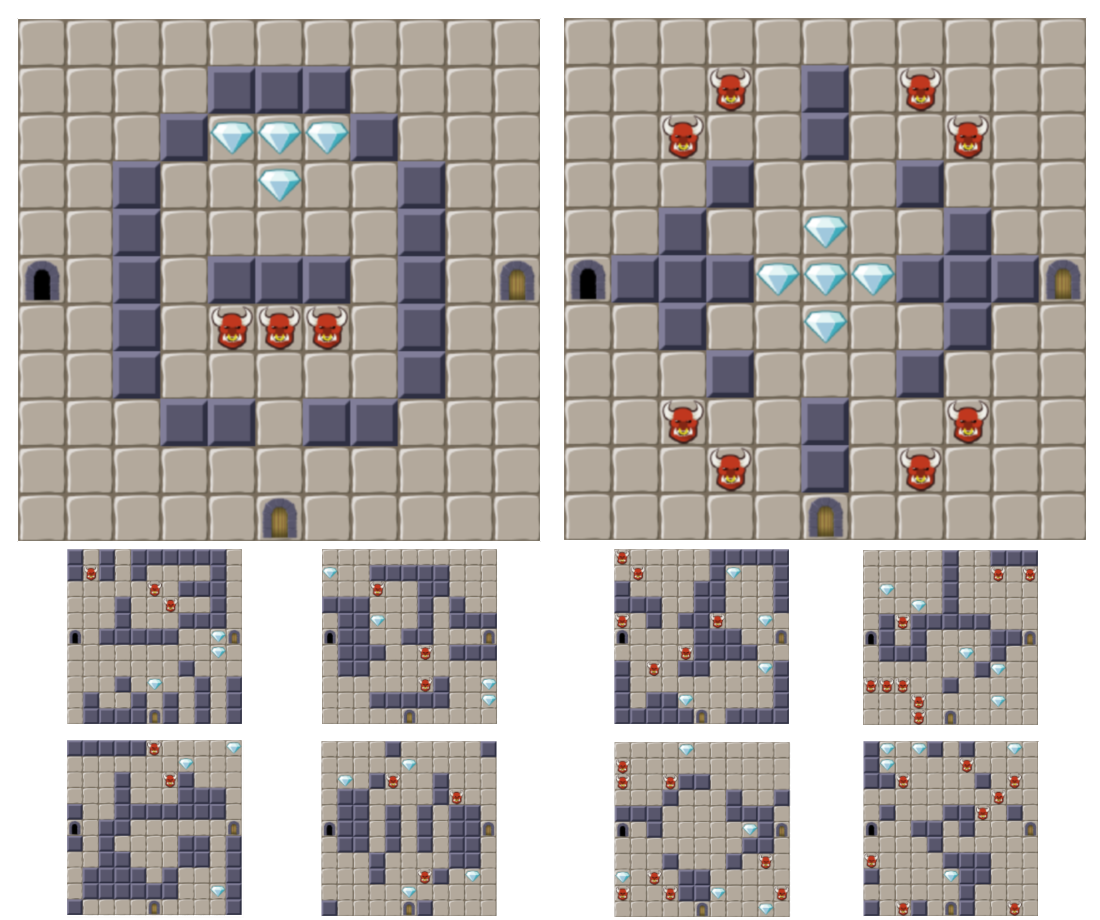
\includegraphics[scale=0.39]{Figures/figure-not-preserving}
% \caption{Sample maps from the previous version of EDD, not preserving the aesthetic changes in suggestions}
% \label{p2fig:no-aesthetic}
% \end{figure}

%The criteria can vary depending on the technique used, the goal to be reached and the evaluation to be performed. In offline generation, the algorithm tries to satisfy functional criteria (e.g. the level can be finished or all the passable tiles are accessible) \citepsecond{p2Shaker2016TheApproach,Togelius2007TowardsGames}. 
\begin{figure} [!h]
\centering
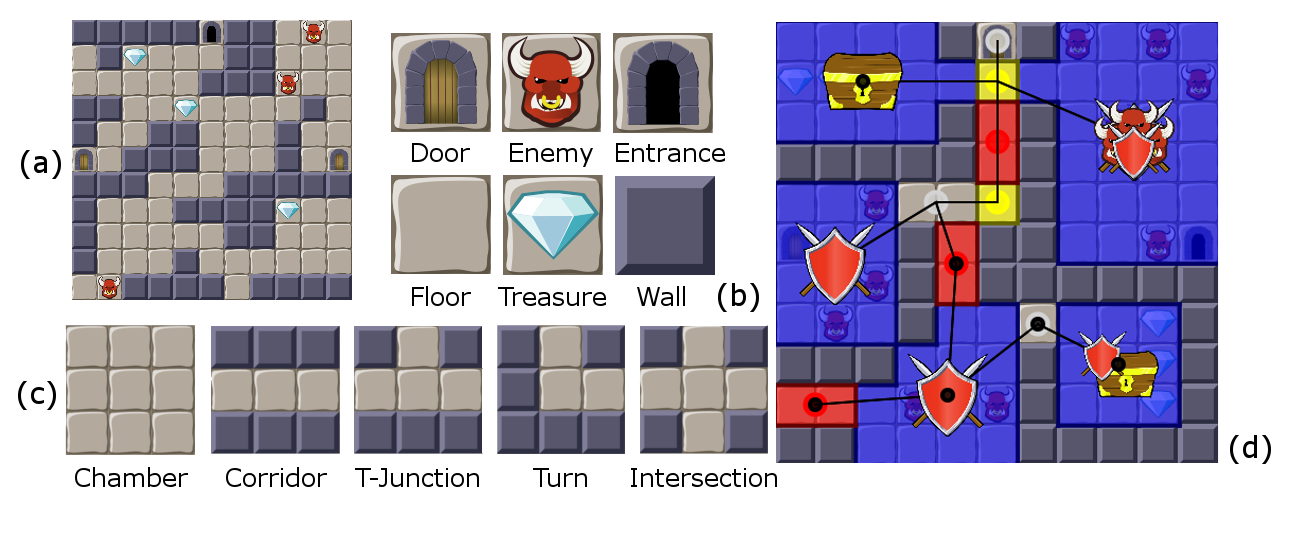
\includegraphics[width=\textwidth]{included-papers-tex/paper-2/pap2-figures/map-figure.png}
\caption{Current version of EDD and its different components. (a) Basic room, (b) different placeable tiles, (c) micro-patterns and (d) meso-patterns.}
\label{p2fig:eddy-map}
\end{figure}

As discussed by~\citepsecond{p2Baldwin2017TowardsGeneration}, it is important for a mixed-initiative SBPCG approach to evaluate the degree to which generated designs are aesthetically pleasing and interesting to the human designer. This is stressed by the designer's will to imprint and preserve their custom designs on the generated content offered by the PCG system. It is a non-trivial task to know which parts the designer wants to preserve, as well as correctly balancing human and procedurally designed content in the generated solutions. This motivates the work presented here, in which we address the need for assessing aesthetic criteria by improving both: the solution encoding mechanism and the fitness evaluation function in EDD's evolutionary algorithm.

%The overall goal of the research is to assess one of the problems that arose from the previous research's case study \citepsecond{p2Baldwin2017TowardsGeneration}, where the generator did not capture and preserve the manually edited changes done by the designers nor their aesthetic criteria in the generated suggestions. as shown in figure \ref{p2fig:no-aesthetic}. 

This paper is organized as follows: Section \ref{p2background} presents previous and related works in mixed-initiative design. Section \ref{p2approach} describes in detail the contributions of this paper and presents the results from the laboratory experiments used for validating them. Finally, Section \ref{p2conclusion} summarizes and discusses these results, as well as sets future questions to be addressed by further research in the area of aesthetic criteria and EDD.

\subsection{Related Work} \label{p2background}

\begin{figure}
\centering
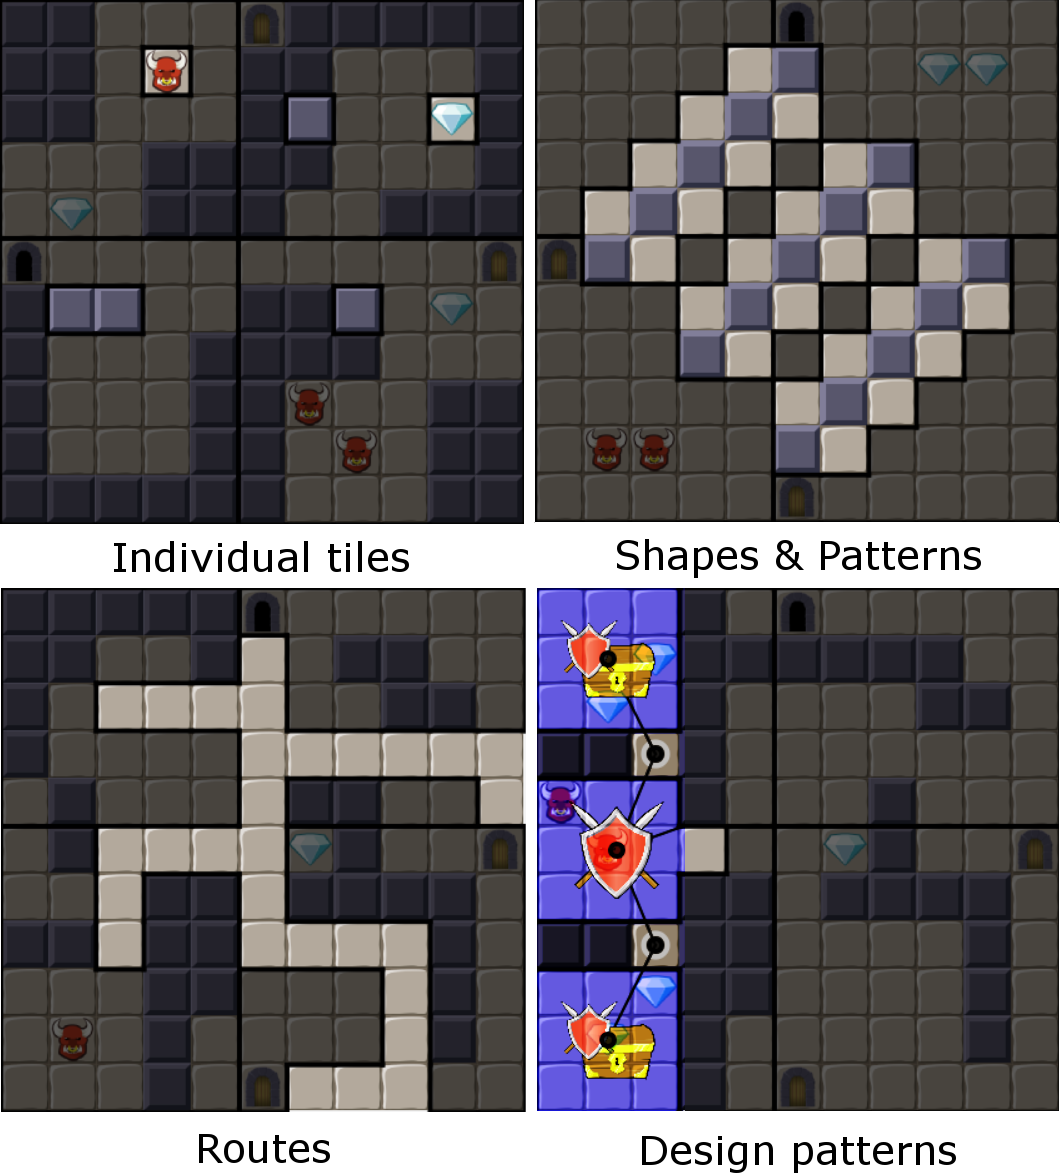
\includegraphics[width=0.7\textwidth]{included-papers-tex/paper-2/pap2-figures/figure-possible-zones.png}
\caption{Different uses and possibilities that the designers can have for locking the tiles in the Room, in order to, preserve their manual changes and diverse objectives}
\label{p2fig:possible-zones}
\end{figure}


Aesthetic criteria was specified by previous research as a key feature while evaluating content, as it leads to the generation of more customized content in the eyes of the human designer, whose aesthetic vision on the content is preserved~\citepsecond{p2Liapis2012AdaptingCreation,p2Hastings2009GalacticGame,p2Machwe2006IntegratingInvestigation}.

%\emph{Tanagra}~\citepsecond{p2Tanagra2011} is used to develop 2D platform levels. The user can place different tiles, and is able to select content, which they want to keep, while Tanagra generates content around them. 

%Aesthetic criteria has been appointed by previous research as a key feature while evaluating content, as it leads to the generation of more customized content to the eyes of the human designer, whose aesthetic vision on the content is preserved \citepsecond{p2Liapis2012AdaptingCreation,Hastings2009GalacticGame,Machwe2006IntegratingInvestigation}.

Interactive evolutionary approaches incorporate human evaluation by allowing the user to select, either implicitly or explicitly, the parents of the next generation of procedurally generated individuals. In~\citepsecond{p2Zhang2015DrawCompileEvolve:Creations} system allows users to draw simple primitive shapes to seed an evolutionary algorithm and train a neural network with their aesthetic vision. In Galactic Arms Race~\citepsecond{p2Hastings2009GalacticGame} players preferences on the evolved weapons is implicitly deducted from the amount time they actively select those weapons during the gameplay.

\citepsecond{p2Liapis2012AdaptingCreation}, incorporated visual aesthetics as an evaluation of their generated spaceships by calculating different aesthetic concepts: symmetry along axes, weight distribution or design simplicity. Moreover, ~\citepsecond{p2Mario2016ACM} generated levels for Mario using symmetry as objective function, which based on their user study, were as visually pleasing as the ones created by human designers and even more than other similar approaches. 

%\citepsecond{p2Liapis2012AdaptingCreation}, incorporated visual aesthetics as an evaluation of their generated spaceships by calculating different aesthetic concepts: symmetry along axes, weight distribution or design simplicity. These were computed to produce the aesthetic fitness of a spaceship, letting the user select their preferred spaceship to adjust the weight of the different aesthetic features in the fitness calculation.


%\begin{itemize}
%  \item EDDY previous versions
%  \item Previous approaches to evaluate aesthetic criteria of the designer
%  \begin{itemize}
%  	\item Aesthetic criteria was seen as visually pleasing for the designer but that does not mean that it is the idea that the user had. For mixed-initiative the way to evaluate aesthetic criteria usually was by allowing the user to select the options that he liked the most  Show examples of Mario level generator and such.
%    \item To preserve Aesthetic criteria other authors have allow the user to initiate the evolutionary algorithm with an example (initial seed) and from there, allow the evolutionary algorithm to produce suggestions based on this.
%  \end{itemize}
%\end{itemize}

%The work presented in this paper is an extension to the ongoing research of EDD \citepsecond{p2Baldwin2017TowardsGeneration} and addresses the issue of preserving manual changes to the level and the impact of visual aesthetic criteria when designing dungeons.

\subsubsection{The Evolutionary Dungeon Designer}

EDD is a mixed-initiative authoring tool for generating dungeon rooms using a feasible-infeasible two population (fi-2pop) evolutionary approach, which is interactively evaluated and edited by a designer. The current version of EDD consists of six different building blocks that represent floors, walls, enemies, treasures, doors and entrances. This can be used by the user to brush paint and compose a NxM size room which, at its minimum, must hold one of each tile. Both the tiles and the finished room can be seen in Figure~\ref{p2fig:eddy-map}a) and b).

EDD takes the work presented in The Evolutionary World Designer~\citepsecond{p2Font2016ConstrainedAlgorithms} one step further, by procedurally generating rooms and their specific content. EDD's EA follows the approach of~\citepsecond{p2Liapis2012AdaptingCreation} using the evaluation of the user to change the internal evaluation and configuration of the system. Its fitness evaluation is driven by the use of game design micro- and meso- patterns, as shown in Figure \ref{p2fig:eddy-map} c) and d). A detailed description of EDD's pattern-based fitness, genetic algorithm and mixed-initiative approach can be found in \citepsecond{p2Baldwin2017Mixed-initiativePatterns} and \citepsecond{p2Baldwin2017TowardsGeneration}.

\subsection{Assessing Aesthetic Criteria} \label{p2approach}

\begin{figure}
\centering
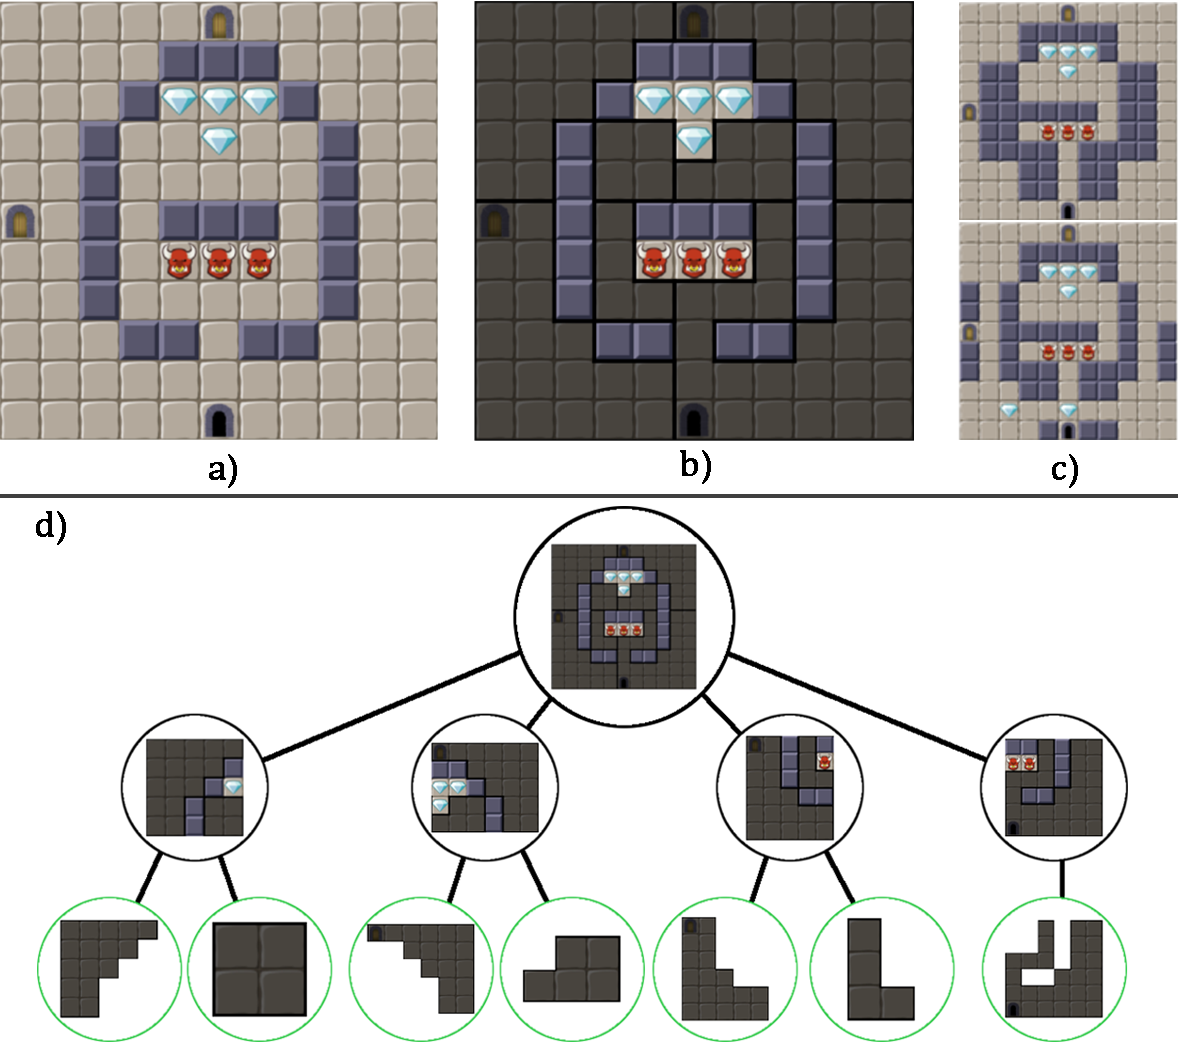
\includegraphics[width=0.7\textwidth]{included-papers-tex/paper-2/pap2-figures/map-representation-figure-test.png}
\caption{A sample edited room (a) with its division into zones (b) based on the tiles locked by the user. Suggestions preserve these locked tiles (c). The room and its zones are internally represented with a tree structure (d), where the leaf nodes (green) are the valid candidates to operate within an individual.}
\label{p2fig:map-representation}
\end{figure}

Our approach is divided in two; on one side, the algorithm implicitly has control over different aesthetic criteria using the edited room as a base to measure symmetry and similarity for the EA. On the other side, the designer was given control over what they wanted to preserve by being able to select tiles in the room to be immutable (i.e. not changeable in following generations).

\subsubsection{Preserving Custom Aesthetic Structures}

%To preserve the aesthetic criteria of a designer's edited room, we give him/her the ability to manually lock custom structures in it, preserving these in the upcoming the next suggestions. This is possible by incorporating a new brush which is used as a complementary modifier when editing the room. The designer can now lock any range of tiles, making it possible to preserve individual tiles, shapes, patterns, routes and even design patterns as shown in Figure \ref{p2fig:possible-zones}. 
To preserve the aesthetic criteria of a designer's edited room, we give the users the ability to manually lock custom structures in it, preserving these in the upcoming suggestions. This is possible by incorporating a new brush which is used as a complementary modifier when editing the room. The designer can now lock any range of tiles, making it possible to preserve individual tiles, shapes, patterns, routes and even design patterns as shown in Figure~\ref{p2fig:possible-zones}.

The process to subdivide the room is straightforward; the designer is presented with the room to be edited, and by using the lock brush, the room seamlessly subdivides and creates zones, which classifies the room's tiles into two sets: the immutable tiles (i.e. invalid or locked) and the mutable tiles (i.e. valid or unlocked).

An individual's genotype is now changed from a direct encoding (each tile is a gene) to a semi-direct encoding using a tree structure, with the nodes of the tree as different zones of the room, constructed from the mutable and immutable tiles, and the leaf nodes, only containing sets of mutable tiles, as candidates to be used for crossing and mutation. Figure~\ref{p2fig:map-representation} shows the room, it's division into zones and the tree representation used by the EA. 

The advantages of this representation are that it allows the EA to reduce the search space by only considering valid zones of the room, and improves the crossover operator by allowing the exchange of irregular shapes between individuals along different parts of the room.

%An individual's genotype is now changed from a direct encoding (each tile is a gene) to a semi-direct encoding using a tree structure, with the nodes of the tree as different sections of the room and the leaf nodes as candidates to be used for crossing and mutation. Figure~\ref{p2fig:map-representation} shows the room, it's division into zones and the tree representation used by the EA. This change in the individual representation improves the crossover operator by allowing the exchange of irregular shapes between individuals along different parts of the room. This results in an increased presence of custom (user-shaped) building blocks among the generated offspring.

In practice, this solution allows users to preserve any aesthetic change (either significant or detailed) that they want to keep in further generations, while still receiving novel suggestions created following the pattern-based fitness function. It also means that the construction of the dungeon can be performed differently: instead of manually editing a room first to later generate appealing solutions based on it, the user can now start from a suggestion, selecting parts of it that look promising that are kept through subsequent generations, until the user's needs and criteria are met.

%In practice, this solution allows users to preserve any aesthetic change (either significant or detailed) that they want to keep in further generations, while still receiving novel suggestions created following the pattern-based fitness function. It also means that the construction of the dungeon can be performed differently: instead of manually editing a room first to later generate appealing solutions based on it, the user can now start from a suggestion, selecting parts of it that look promising that are kept through the following generations of procedurally generated suggestions, until the user's needs and criteria are met.

%In practice, this solution allows users to preserve any aesthetic change (either significant or detailed) that they want to keep in further generations, while still receiving novel suggestions created following the pattern-based fitness function. It also means that the construction of the dungeon can be performed differently: instead of manually editing a room first to later generate appealing solutions based on it, the user can now start from a suggestion, selecting parts of it that look promising that are kept through the following generations of procedurally generated suggestions, until one meets his/her needs and criteria.

\subsubsection{Evaluating Symmetry and Similarity}

\begin{figure}
\centering
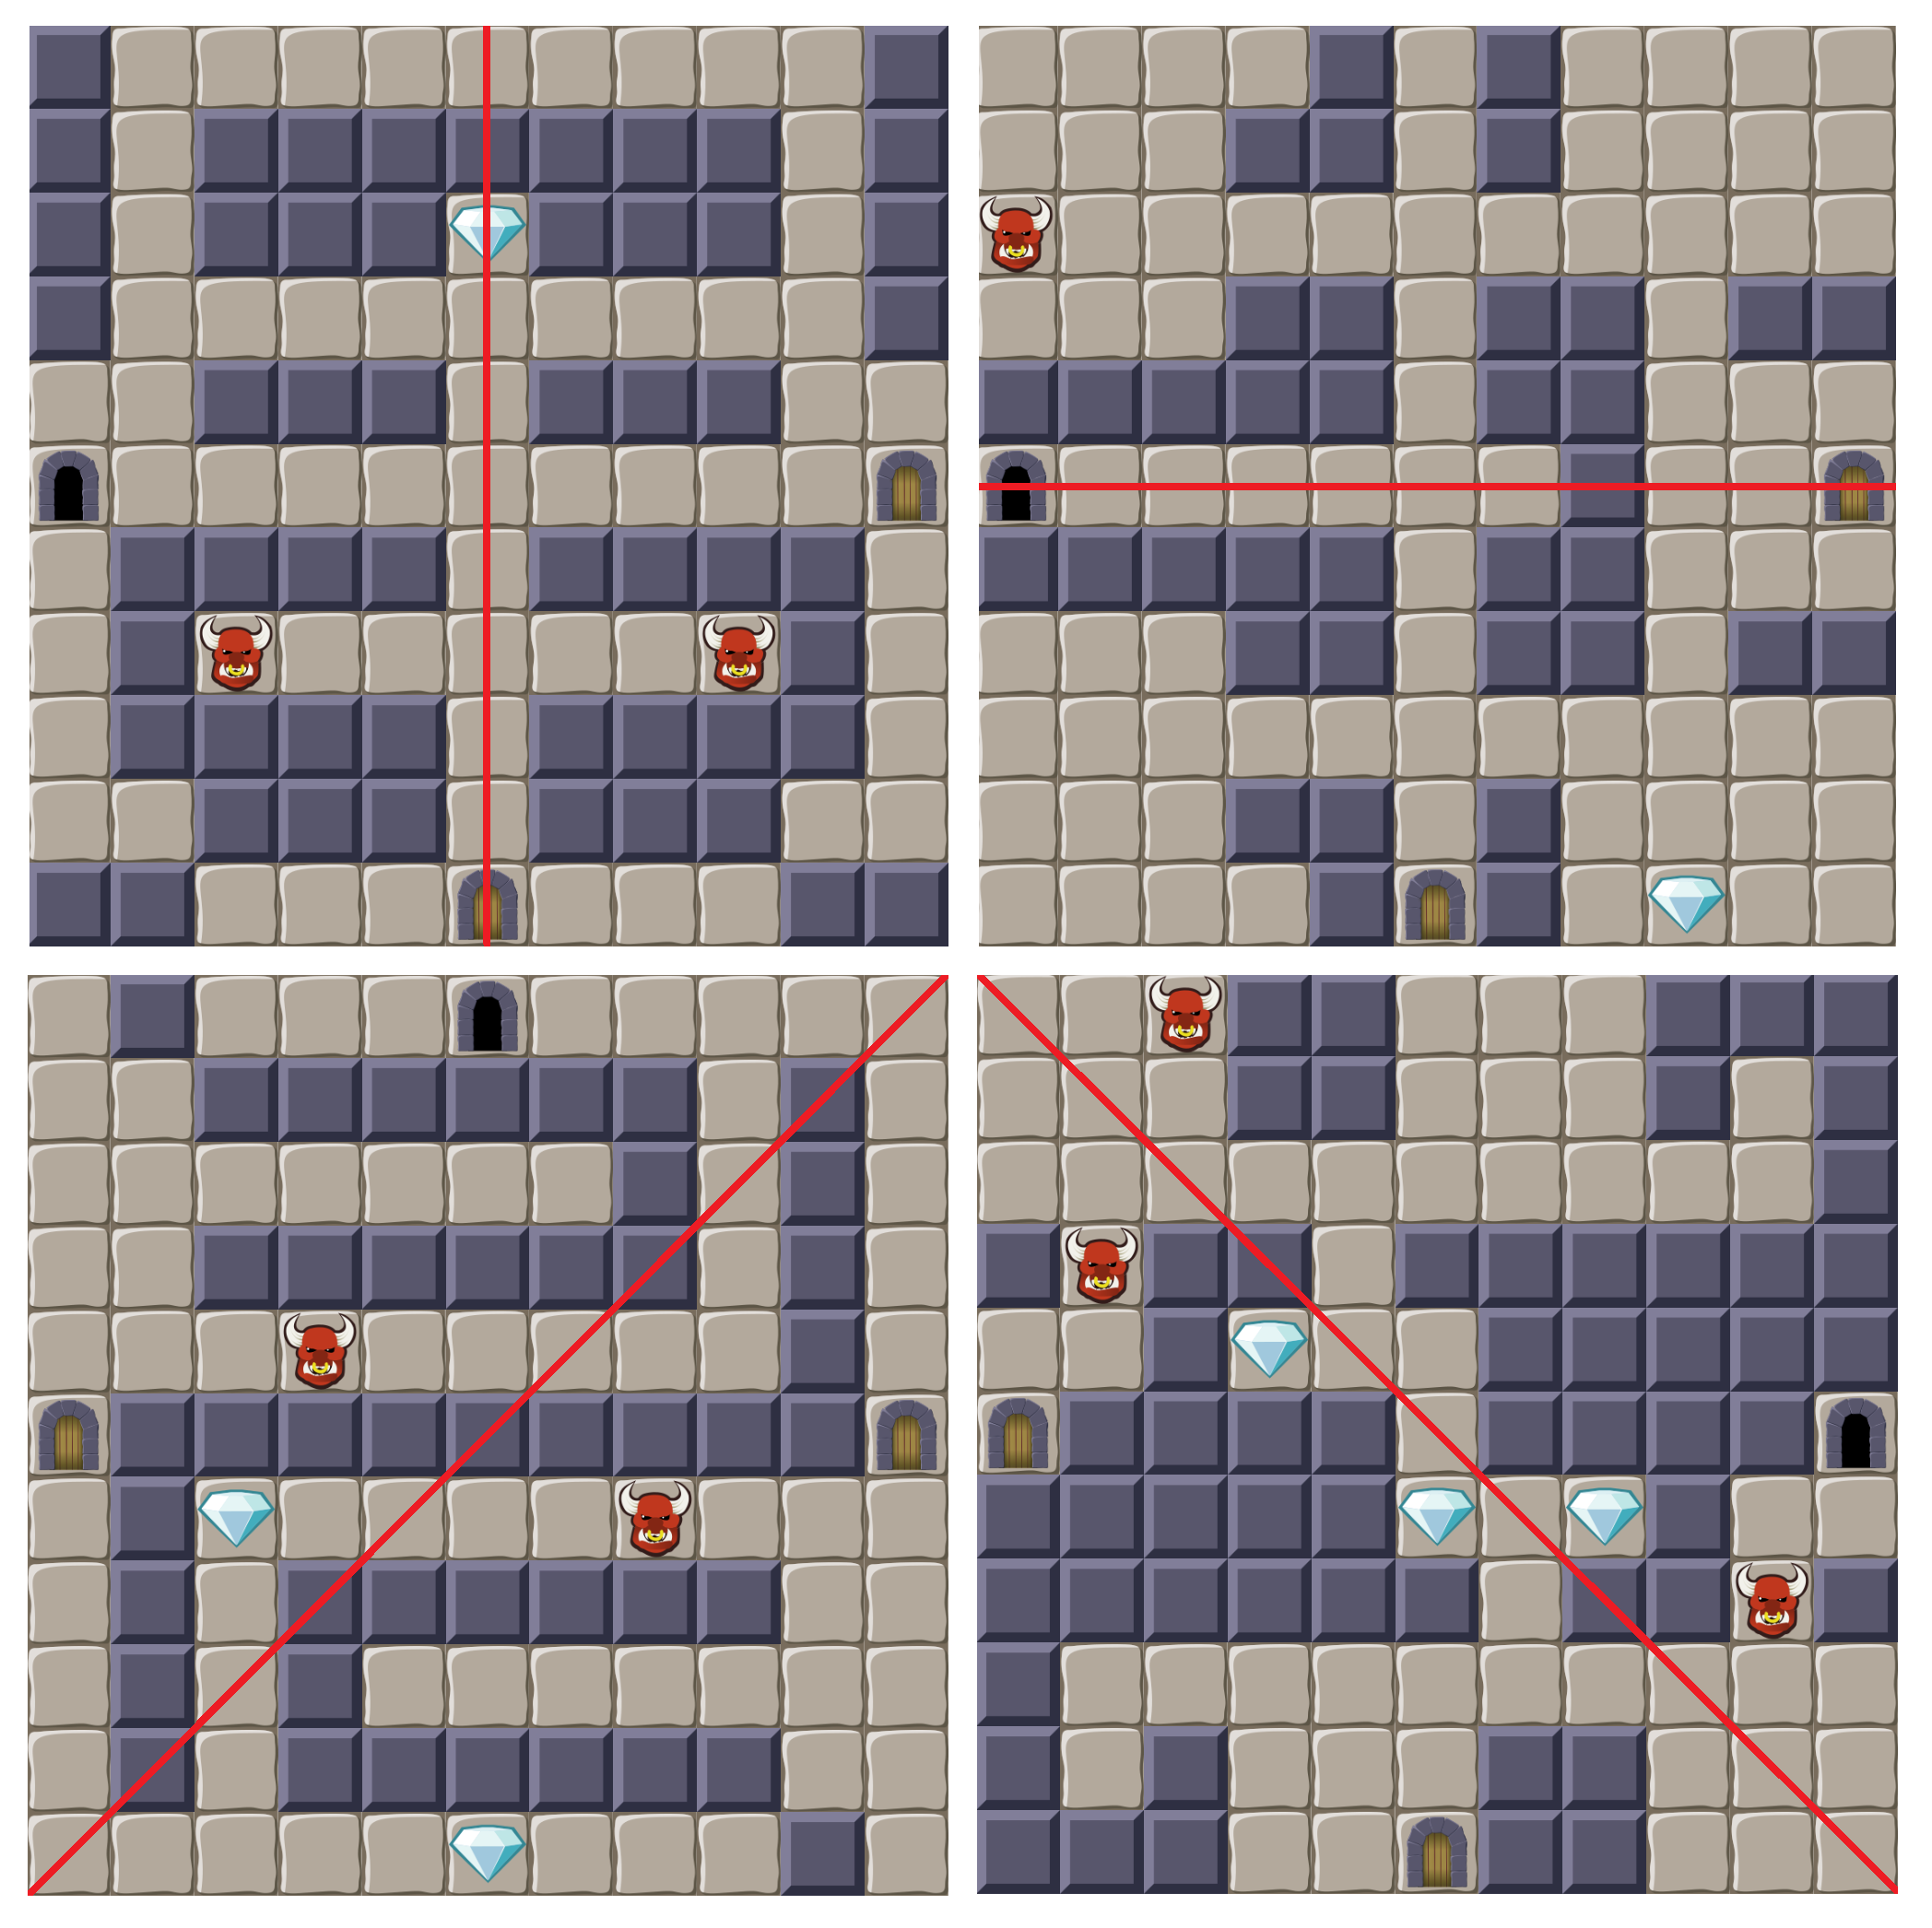
\includegraphics[width=0.7\textwidth]{included-papers-tex/paper-2/pap2-figures/DifferentSymmetry.png}
\caption{Different types of symmetry evaluated}
\label{p2fig:symmetry-types}
\end{figure}

While the pattern-based fitness function worked well for functionality purposes, it did not consider nor capture any aesthetic aspects into it. Therefore, in order to consider and preserve visual aesthetic criteria, we evaluate the rooms for their symmetry  along the X and Y axes, backslash and front slash diagonal as shown in Figure \ref{p2fig:symmetry-types} and calculate the similarity that subsequent individuals had in comparison with the original edited room. For simplicity, we differentiate the room by impassable (i.e. walls) and passable (i.e. floor, treasure and enemy) tiles.

%In order to implicitly consider and preserve visual aesthetics criteria, we evaluate the rooms for their symmetry  along the X and Y axes, backslash and front slash diagonal as shown in Figure \ref{p2fig:symmetry-types} and calculate the similarity that subsequent individuals had in comparison with the original edited room. For simplicity, we differentiate the room by impassable (i.e. walls) and passable (i.e. floor, treasure and enemy) tiles.

%In order to implicitly consider and preserve visual aesthetics criteria, we evaluated the rooms for their symmetry  along the X and Y axes, backslash and front slash diagonal as shown in Figure \ref{p2fig:symmetry-types} and calculated the similarity that subsequent individuals had regarding the original edited room. For simplicity, we differentiated the room by unpassable (i.e. walls) and passable (i.e. floor, treasure and enemy) tiles.

\paragraph{Symmetry evaluation}

%unpassable
%To calculate the symmetry of a room we evaluate the impassable tiles of one side against their corresponding tile on the other side for the X and Y axes and diagonals. The highest symmetric value is then used to calculate a curve ranging from 0 to 1, using equation \ref{p2eq:Symmetry}.

To calculate the symmetry of a room we evaluate the impassable tiles of one side against their corresponding tile on the other side for the X and Y axes and diagonals. The highest symmetric value is then used in equation~\ref{p2eq:Symmetry} to calculate the fitness.

\begin{equation} \label{p2eq:Symmetry}
f_{symmetry} = \frac{highestSymmetricValue} {totalWalls}
\end{equation}

Equation~\ref{p2eq:Symmetry} allow us to calculate symmetry while also preventing the favoring of more walls. Once calculated, we weight the result into the individual's fitness, and as consequence it would favor more or less symmetric rooms and preserve the room's configuration as it can be seen in Figure~\ref{p2fig:symmetry-result}.

\begin{figure}
\centering
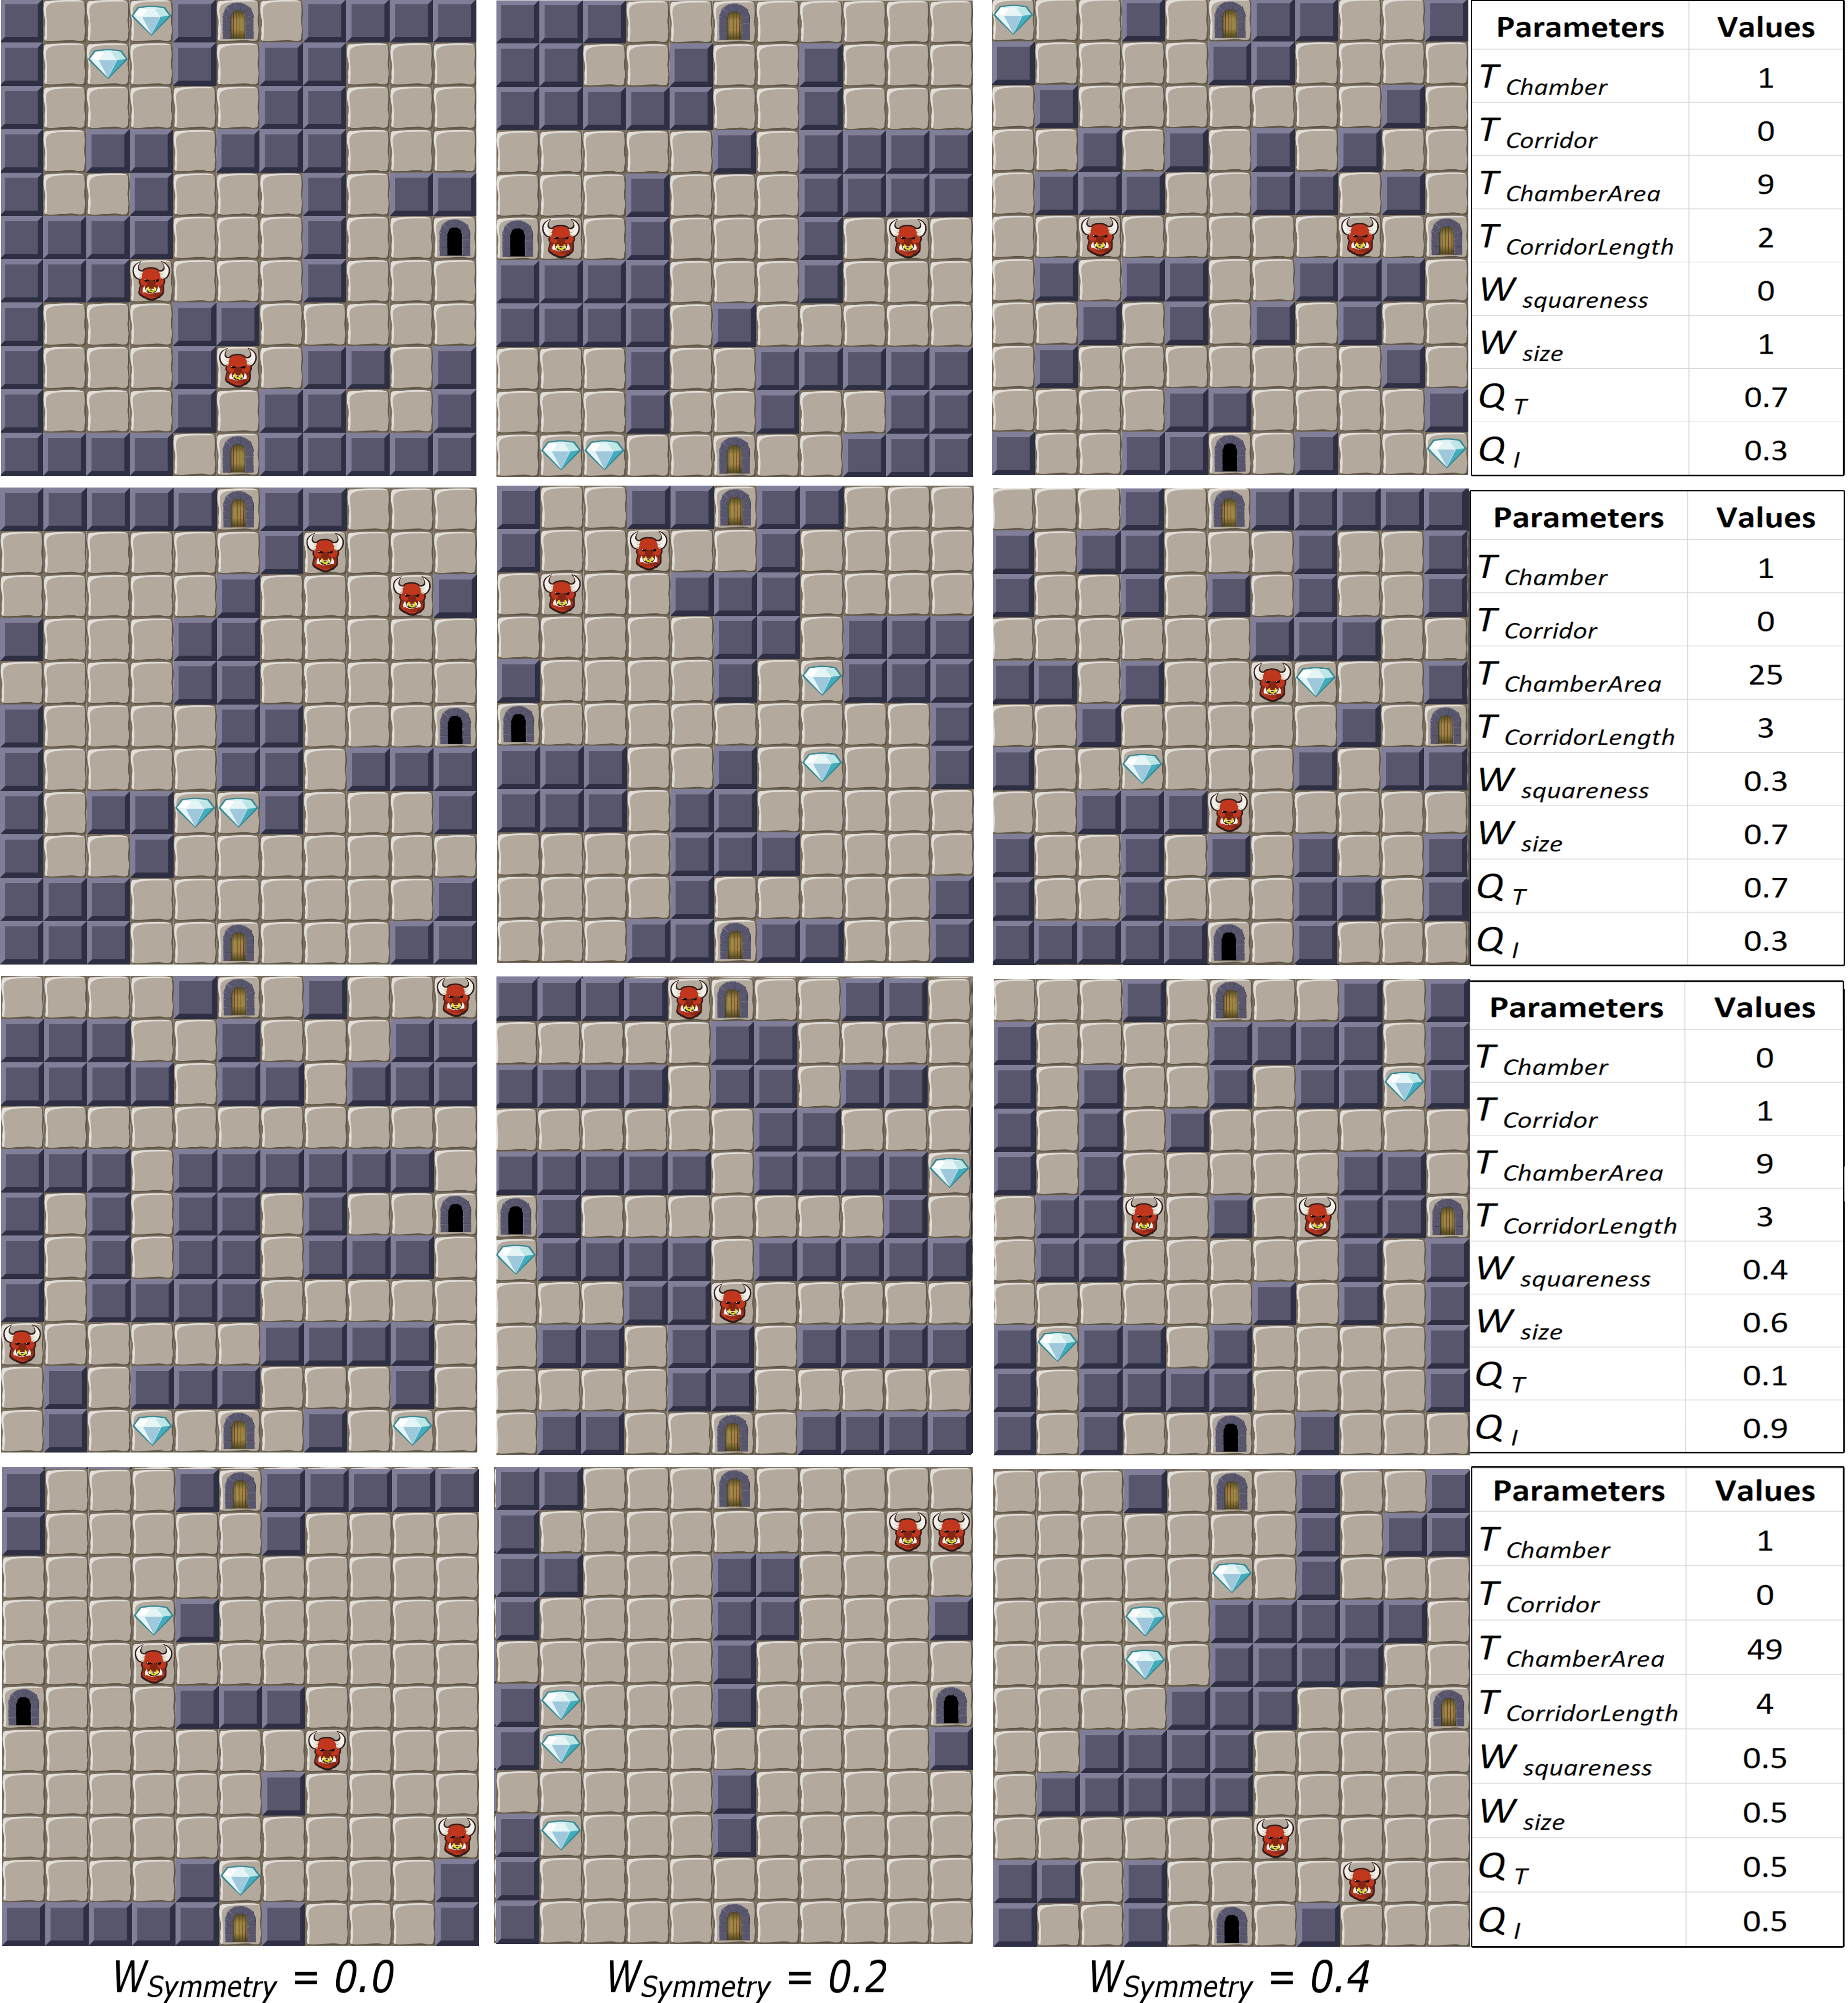
\includegraphics[width=0.7\textwidth]{included-papers-tex/paper-2/pap2-figures/symmetry-result-figuer.png}
\caption{Each row shows three results (\(W_{symmetry}=0, W_{symmetry}=0.2, W_{symmetry}=0.4\) ) produced under the settings displayed on the rightmost column. Metrics adapted from~\protect\citepsecond{p2Baldwin2017Mixed-initiativePatterns}.}
\label{p2fig:symmetry-result}
\end{figure}

\paragraph{Similarity evaluation}

The similarity value between an edited room and successive evolved rooms is calculated by comparing every tile in the original with the corresponding tile in subsequent individuals. Once the total amount of equal tiles is known, we calculate the similarity percentage based on the total amount of tiles, following equation~\ref{p2eq:ProcentSimilar}. 

\begin{equation} \label{p2eq:ProcentSimilar}
similarityPercentage = \frac{totalTiles - notSimilarTiles} {totalTiles}
\end{equation}

%In order for the similarity percentage to be useful we introduced \(idealSimilarityPercentage\) as a parameter related to how similar we want the individuals to be, and use it to normalize the final \(f_{similarity}\) as shown in equation~\ref{p2eq:FSimilarity} or if \(SimilarityPercentage\) was higher then we use~\ref{p2eq:FSimilarity2}.

%\begin{equation} \label{p2eq:FSimilarity}
%f_{similarity} = \frac{SimilarityPercentage} {idealSimilarityPercentage}
%\end{equation}

%\begin{equation} \label{p2eq:FSimilarity2}
%f_{similarity} = \frac{1 - SimilarityPercentage} {1 - idealSimilarityPercentage}
%\end{equation}

We introduced a second parameter called \(idealSimilarity\), which represents how similar we want the individuals to be. Following equation~\ref{p2eq:FSimilarity} we measured the error between both similarities and used it as the similarity fitness. 

\begin{equation} \label{p2eq:FSimilarity}
f_{similarity} = 1 - \left |idealSimilarity - SimilarityPercentage \right |
\end{equation}

The result of incorporating the similarity evaluation into the final fitness is shown in Figure~\ref{p2fig:similarity-result} where is observable that depending on the \(idealSimilarityPercentage\) the original room goes from having a slight variation to start losing its resemblance.

\begin{figure}
\centering
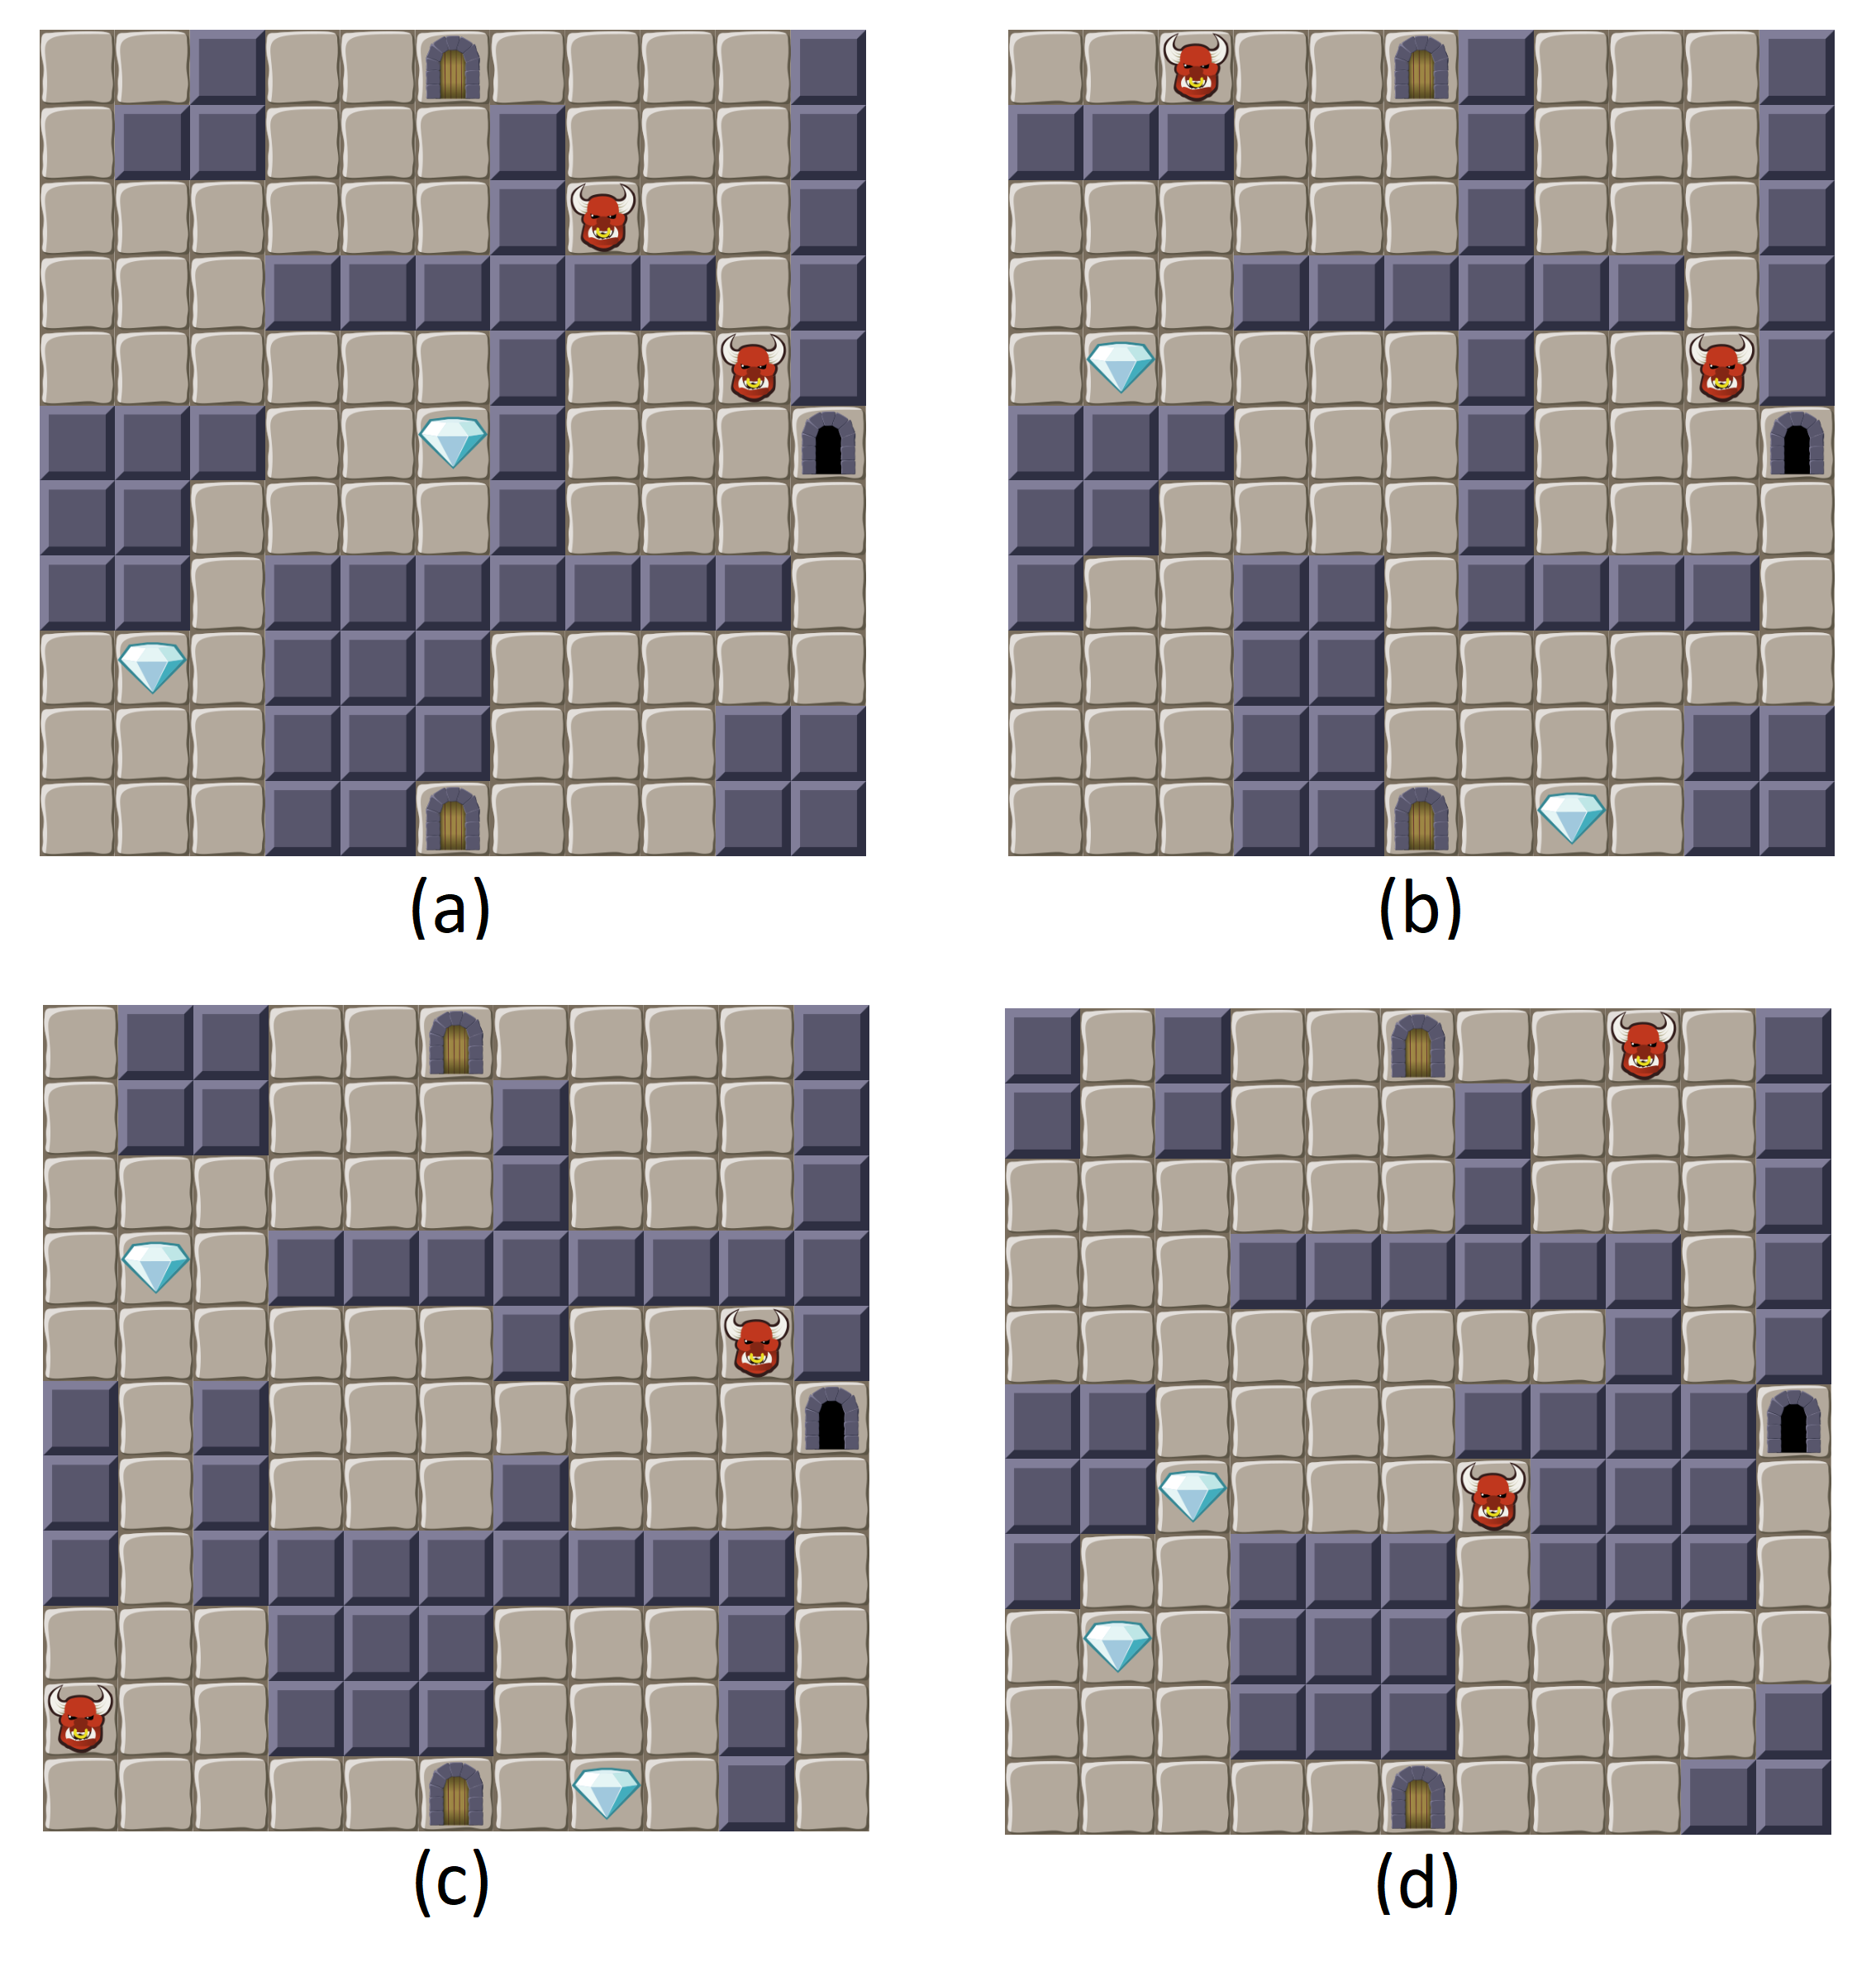
\includegraphics[width=0.7\textwidth]{included-papers-tex/paper-2/pap2-figures/figure-similarity.png}
\caption{(a) Sample original room and the evolved solutions with different \(idealSimilarity\) values in order: (b)~0.95, (c) 0.90 and (d) 0.85.}
\label{p2fig:similarity-result}
\end{figure}

Finally and expanding over the previous work on EDD~\citepsecond{p2Baldwin2017TowardsGeneration}, these calculations (i.e. \(f_{symmetry}\) and \(f_{similarity}\)) are included into the existing fitness evaluation of an individual as shown in equation \ref{p2eq:SiSyFitness}. \(f_{inventorial}\) and \(f_{spacial}\), evaluates the overall layout of the room, and the frequency and quality of the design patterns in the room, respectively. An in-depth explanation of both can be found in~\citepsecond{p2Baldwin2017TowardsGeneration}.

%Finally and expanding over the previous work on EDD~\citepsecond{p2Baldwin2017TowardsGeneration}, these calculations are included into the existing fitness evaluation of an individual as shown in equation \ref{p2eq:SiSyFitness}.

\begin{equation} \label{p2eq:SiSyFitness}
\begin{split}
f_{fitness}(r) & = (\frac{a}{10}f_{inventorial}(r) \,+ \, \frac{b}{10}f_{spacial}(r) \\ 
 & \, + \; \frac{c}{10}f_{symmetry}(r)) \ * \ f_{similarity}(r)
\end{split}
\end{equation}

\subsection{Conclusions and Future Work} \label{p2conclusion}

In this paper, we have presented the advancements done on EDD in relation to the evolutionary system with different evaluations, encoding, genotype representation and strategies that aims on preserving and consider the designer's aesthetic criteria.

By introducing the capability of locking sections of a room, we changed the individual's encoding from direct to semi-direct, and in turn, offered new and easier possibilities to perform different operations to the individuals, as well as, allowing the designer to preserve individual tiles, shapes, routes and even design patterns.

%By changing the encoding of the evolutionary algorithm from direct to semi-direct encoding we opened the possibilities to perform different operations to the individuals, as well as a fair way of preserving the sections of the map which were considered important, significant and unchangeable by the designer. As result, the generator has increased on controllability at expenses of expressiveness. Moreover, this approach allows the designer not only to lock and preserve interesting aesthetical changes done in the map but also indirectly, is able to preserve routes and design patterns.

Moreover, we successfully integrated and produced rooms evaluated  on symmetry and similarity that held the overlying structure of the micro-patterns. The added evaluations establishes the path to preserve and consider more in-depth the designers criteria and produce personalized work that accurately transmit the ideas and intentions of the designer.

%In the end, we successfully integrated and produced dungeon levels which, held the overlying structure of the micro-patterns and symmetry together \textbf{(here is missing the part of the similarity)}. Moreover, the added evaluations to the fitness of each individual allows us to establish the path to preserve and consider more in-depth the designers criteria and produce a more personalized work that accurately transmit the ideas and intentions of the designer.

We aim to more throughly evaluate the system by incorporate the three techniques into a user study, similar to the one done by~\citepsecond{p2Baldwin2017TowardsGeneration} to validate the tool's capacity on assessing the designer's criteria. It would be interesting to add more aesthetic concepts to evaluate the produced content, for instance, density, simplicity, sparseness and individuality.

%We aim to further evaluate the system with different configurations and observe how the different fitness functions can interact and cooperate with each other to create more interesting content, as well as, joining both approaches for a case study, similar to the one done by Baldwin et al \citepsecond{p2Baldwin2017TowardsGeneration}. It would be interesting to continue using aesthetic concepts, for instance, density, simplicity, sparseness and individuality, to evaluate the content 

The subdivision of the map could be extended to perform a parallel evolution on the custom aesthetic structures locked by the designers and propose interesting variations. Moreover, a zone analysis could be introduced to increase the dungeon's knowledge for the designer by suggesting changes to fulfill different player models, similar to Holmg\r{a}rd's approach~\citepsecond{p2Holmgard2014EvolvingModeling}, or paths and statistics. Finally, we would like to explore different types of representations towards more generative encodings to test, compare and measure the differences and advantages of the resulting maps.

%Further use the division of the map by performing zone analysis, which could result on suggesting changes to the designers in order to fulfill different player models, similar to Holmg\r{a}rd's approach \citepsecond{p2Holmgard2014EvolvingModeling} or do a separated evolution on the manually locked tiles providing the designers with interesting shapes and patterns. Finally, we would like to go down the road towards more indirect encodings and test different approaches and, compare and measure the differences and advantages of the resulting maps.

%\subsection{Future Work} \label{p2future-work}

We aim to further evaluate the system with different configurations and observe how the different fitness functions can interact and cooperate with each other to create more interesting content, as well as, joining both approaches for a case study, similar to the one done by Baldwin et al \citepsecond{p2Baldwin2017TowardsGeneration}. It would be interesting to continue using aesthetic concepts, for instance, density, simplicity, sparseness and individuality, to evaluate the content 

Further use the division of the map by performing zone analysis, which could result on suggesting changes to the designers in order to fulfill different player models, similar to Holmg\r{a}rd's approach \citepsecond{p2Holmgard2014EvolvingModeling} or do a separated evolution on the manually locked tiles providing the designers with interesting shapes and patterns. Finally, we would like to go down the road towards more indirect encodings and test different approaches and, compare and measure the differences and advantages of the resulting maps.